\begin{figure}[!htb]
\centering
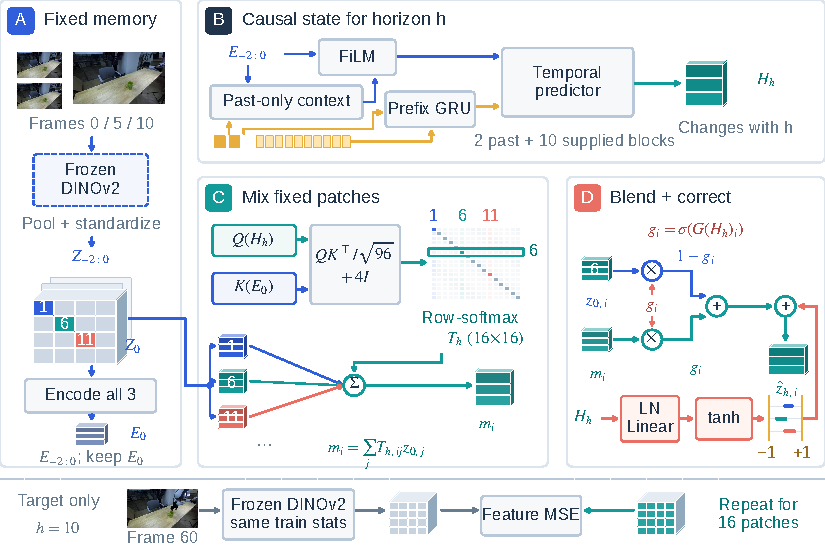
\includegraphics[width=\linewidth]{generated/editorial/architecture_visual_design.pdf}
\caption[ShiftWM observed-memory architecture.]{\textbf{ShiftWM: the proposed decoder is the fixed-source mixer and gated correction (C--D).} DINOv2 and the LeWM temporal backbone are reused; the illustrated correction bound is removed in the no-$\tanh$ ablation. (A) Recorded DROID frames 0/5/10 become three frozen-DINOv2 grids with fixed training-only channel normalization. The learned spatial encoder processes all three grids into $E_{-2:0}$; its last pre-FiLM encoding $E_0$ and source $Z_0$ stay fixed throughout forecasting. Only DINOv2 weights are frozen. (B) Context from patch means, their chronological differences and past commands conditions the three encodings; a separate chronological action GRU and temporal predictor produce $H_h$ from the supplied prefix. (C) $Q(H_h)$ and $K(E_0)$ determine a row-softmax matrix with the $+4I$ bias outside $\sqrt{96}$ scaling. The highlighted row $i=6$ mixes all sixteen observed patch vectors; one-based contributors 1/6/11 are illustrated and patch 6 supplies the direct branch in (D). (D) The same $H_h$ sets the affine sigmoid gate and, independently, a LayerNorm--affine $96\!\to\!384$ projection followed by $\tanh$. The complementary blend receives this unit-bounded update in standardized feature coordinates after summation; see Eqs.~\eqref{eq:editorial-mixing}--\eqref{eq:editorial-forecast}. The lower lane scores the assembled feature grid against the withheld frame through the same frozen encoder and normalization, with no target-to-predictor path. Feature pieces, weights and channel bars are schematic, not RGB forecasts. DROID photographs are unchanged (CC BY 4.0).}
\label{fig:editorial-spatial-method}
\end{figure}
